% !TeX root = RJwrapper.tex

\title{\pkg{rotations}: A Package for $SO(3)$ Data}
\author{by Bryan Stanfill, Heike Hofmann, Ulrike Genschel}

\maketitle

\abstract{
In this article we introduce the \pkg{rotations} package which provides users with the ability to simulate, analyze and visualize three-dimensional rotation data.  The \pkg{rotations} package gives the user access to four distributions from which to simulate data, four estimators of the central orientation, three confidence region estimation procedures and a novel approach to visualizing these data.  All of the above features are available to two different parameterizations of rotations: three-by-three matrices and quaternions.
}

\section{Introduction}

Data in form of three-dimensional rotations find application in several scientific areas, such as bio-medical engineering, computer visioning, and geological and materials sciences where such data represent the positions of objects within some three-dimensional reference frame.  For example, \cite{humbert1996, bingham2009, bachmann2010} use rotation data to study the orientation of cubic crystals on the surfaces of metal.  \cite{rancourt2000} use this data to represent an individual's body position while performing a task. 

A common goal shared by these fields is to estimate the main or central orientation for a sample of rotations.  That is, letting the rotation group $SO(3)$ denote the collection of all $3\times 3$ rotation matrices, observations $\bm{R}_1,\ldots,\bm{R}_n \in SO(3)$ can be conceptualized as a random sample from a \textit{location model}
\begin{equation}
\label{eqn:loc_model}
\mathbf{R}_i = \bm{S} \bm{E}_i, \quad i=1,\ldots,n,
\end{equation}
where $\bm S \in SO(3)$ is the {\it fixed} parameter of interest indicating an orientation of central tendency, and $\bm{E}_1,\ldots,\bm{E}_n \in SO(3)$ denote i.i.d. {\it random} rotations which symmetrically perturb $\bm{S}$.  The data-generating model in \eqref{eqn:loc_model} is a rotation-matrix analog of a location model for scalar data $Y_i = \mu + e_i$, where $\mu \in \mathbb{R}$ denotes a mean and $e_i \in \mathbb{R}$ denotes an additive error symmetrically distributed around zero.

There are a multitude of packages available in R that will estimate the mean in a location model, but for the case of $SO(3)$ data the toolbox is limited.  The \CRANpkg{orientlib} package includes the definition of an orientation class along with a few methods to summarize and visualize rotation data \citep{murdoch2003}.  A strength of the \CRANpkg{orientlib} package is its thorough exploration of rotation representations, but no methods for inference are available and the estimation and visualization techniques are lacking.  The \pkg{uarsbayes} package includes functions for data generation and Bayes inference but is not publicly available \citet{qu2013}.  There are several packages for circular and spherical data, e.g. \CRANpkg{circular} and \CRANpkg{SpherWave}, but their extension to rotation data is non-trivial.

The \pkg{rotations} package fills this void by providing users with the tools necessary to simulate rotations from \eqref{eqn:loc_model} with several distributional models for the perturbation matrices $\bm E_i$.  Estimation and inference for $\bm{S}$ in \eqref{eqn:loc_model} is also available along with novel visualization techniques.  The remainder of this manuscript introduces rotation data more fully and discusses the ways they are handled by the \pkg{rotations} package.


\section{Rotation Parameterizations}

Several parameterizations of rotations exist, we consider two of the most popular: matrices in $SO(3)$ and four-dimensional unit vectors called \dfn{quaternions}.  

\subsection{Matrix Form}

Rotations in three-dimensions can be represented by $3\times3$ orthogonal matrices with determinant one.  Matrices with these characteristics form a group called the \dfn{special orthogonal group}, or \dfn{rotation group}, denoted $SO(3)$.  Every element in $SO(3)$ is associated with a skew-symmetric matrix $\Phi(\bm w)$ where
\[
\bm{\Phi}(\bm{w}) = \left(\begin{array}{ccc}0 & -w_3 & w_2 \\ w_3 & 0 & -w_1 \\-w_2 & w_1 & 0\end{array}\right)
\]
and $\bm w\in\mathbb{R}^3$.  Applying the exponential operator to the matrix $\Phi(\bm w)$ results in the rotation $\bm R$

\begin{equation}\label{eqn:angleaxis}
  \bm R=\exp[\bm{\Phi}(\bm{w})] = \sum\limits_{k=0}^\infty \frac{[\bm{\Phi}(\bm{w})]^k}{k!}=\cos(r)\bm{I}_{3\times3} + \sin(r) \bm{\Phi}(\bm{u}) + [1-\cos (r)] \bm{u} \bm{u}^\top
\end{equation}
where $r=\|\bm{w}\|_F$, $\bm{u} =\bm{w}/\|\bm{w}\|_F$ and $\|\cdot\|_F$ the Frobenius norm.  In the material sciences literature the values $r$ and  $\bm u\in\Rbb^3$ are termed the \dfn{misorientation angle} and \dfn{misorientation axis}, respectively. For more details on this construction see Stanfill et al. (2013) (or some other reference). 

The function \code{SO3} creates a rotation matrix according to \eqref{eqn:angleaxis} for a variety of inputs.  Given an angle and axis \code{SO3} will form a matrix according to \eqref{eqn:angleaxis}; given only a three-dimensional vector the length of that vector will be taken to be the angle of rotation and the vector will be made unit length.  One can also supply a rotation in the quaternion representation and the matrix equivalent will be return as an \code{SO3} object.  A rotation matrix is returned in vector form with class \code{"SO3"} as the following code illustrates for the axis $u=(0, 1, 0)$ and an angle chosen uniformly on the interval $[0,\pi]$.

\begin{example}
> r <- runif(1, 0 , pi) 
> r
2.546667
> u <- c(0, 1 ,0)
> w <- u*r
> R <- SO3(w)
> R
      [,1] [,2]  [,3] [,4] [,5][,6]  [,7] [,8]  [,9]
[1,] -0.82    0 -0.56    0    1    0 0.56    0 -0.82
attr(,"class")
[1] "SO3"
> SO3(u, r)
      [,1] [,2]  [,3] [,4] [,5][,6]  [,7] [,8]  [,9]
[1,] -0.82    0 -0.56    0    1    0 0.56    0 -0.82
attr(,"class")
[1] "SO3"
\end{example}

Moving in the other direction, the functions \code{angle} and \code{axis2} will determine the misorientation angle and axis of a \code{SO3} object.  The code below illustrates that for the rotation \code{R} just constructed the correct angle and axis are computed.
\begin{example}
> angle(R)
2.546667
> axis2(R)
     [,1] [,2] [,3]
[1,]    0    1    0
\end{example}

\subsection{Quaternion Form}

One can also represent a rotation as a unit vector in $\Rbb^4$ called a quaternion.  Quaternions are a form of imaginary numbers with one real entry and a vector of three imaginary parts that can be expressed as
\[
q = x_1 + x_2 i + x_3 j + x_4 k
\]
where $i,j,$ and $k$ are square roots of -1, i.e. $i^2 = j^2= k^2 = -1$.  We can write $\bm q=(s,\bm v)$ as tuple of the scalar $s$ for coefficient $\bm 1$ and vector $\bm v$ for the imaginary coefficients, i.e. $s=x_1$ and $\bm v= (x_2, x_3, x_4)$.

A rotation around axis $\bm u$ by angle $r$ translates to $\bm q=(s,\bm v)$ with
\[
s = \cos{(r/2)},  \ \ \bm v = \bm u \sin {(r/2)}
\]
The following code creates the same rotation from the previous section in the form of a quaternion with the \code{Q4} function.  This function works much the same way as the \code{SO3} function in terms of possible inputs but returns a vector of length four of the class \code{"Q4"}. 

\begin{example}
> Q4(r, u)
     [,1] [,2] [,3]  [,4]
[1,] 0.29    0 0.95     0
attr(,"class")
[1] "Q4"
> Q4(SO3(r, u))
     [,1] [,2] [,3]  [,4]
[1,] 0.29    0 0.95     0
attr(,"class")
[1] "Q4"
\end{example}

%For the remainder of this manuscript only the matrix parametrization will be considered though all the functions are available for quaternions as well.

\section{Data generation\label{section:generation}} 

If the rotation $\bm{E}_i\in SO(3)$ from \eqref{eqn:loc_model} has an axis $\bm u$ that is uniformly distributed on the unit sphere and an angle $r$ that is distributed about $0$ according to some symmetric distribution function then $\bm E_i$ is said to belong to the \dfn{uniform-axis random spin}, or \dfn{UARS}, class of distributions.   From \cite{bingham2009} the density for $\bm E_i$ is given by
\begin{equation}\label{eq:uarsden}
f(\bm E_i|\kappa)=\frac{4\pi}{3-\tr(\bm E_i)}C\left(\left.\cos^{-1}\left\{\frac{1}{2}[\tr(\bm E_i)-1]\right\}\right|\kappa\right)
\end{equation}
where $C(\cdot|\kappa)$ is distribution function connected to the angle of rotation $r$.  Members of the UARS family of distributions are distinguished based on the angular distribution.


The \pkg{rotations} package allows the user access to four members of the UARS class.  Each member is differentiated by the distribution function for $r$: the uniform distribution on the circle, the matrix Fisher \citep{langevin2005, downs1972, khatri1977, jupp1979}, the Cayley  \citep{Schaeben1997, leon2006} and a circular-von Mises-based distribution \citep{bingham2009}.  The uniform distribution on the sphere also plays the role of a uniform measure for $SO(3)$ called the Haar measure.  

The spread of  the Cayley, matrix Fisher and circular-von Mises distributions is controlled by the concentration parameter $\kappa$, but two distributions with the same concentration do not necessarily have the same spread, i.e. a sample from Cayley distribution with $\kappa=1$ is usually more variable than a sample from the matrix Fisher distribution with $\kappa=1$.  To make comparisons across distribution possible we also allow for specification of the circular variance, which is defined as $\nu=1-E[\cos(r)]$ where $E[\cos(r)]$ is called in the circular data literature the \dfn{mean resultant length} \citep{fisher1996}.    The form of each angular distribution along with the circular variance at a function of the concentration parameter is given in Table \ref{tab:Crforms}.

%\begin{center} 
\begin{table}[h!]
\caption{Circular densities with respect to the Lebesgue measure and circular variance $\nu$.}  \label{tab:Crforms}\centering
\small{
\begin{tabular}{ lclclcl}\toprule
\textbf{Name}  & & \textbf{Density} $C(r |\kappa)$ & & \textbf{Circular variance $\nu$}& & \textbf{Function}\\ \midrule 
%\rule[2mm]{0mm}{6mm} 
Uniform  & & $\frac{1-\cos(r)}{2\pi}$ & & $\frac{3}{2}$& & \code{-haar} \\

\rule[2mm]{0mm}{6mm} Cayley  & & $\frac{\Gamma(\kappa+2)(1+\cos r)^\kappa(1-\cos r)}{2^{(\kappa+1)}\sqrt{\pi}\Gamma(\kappa+1/2)}$ & & $\frac{3}
{\kappa+2}$ & & \code{-cayley}\\

\rule[2mm]{0mm}{6mm} matrix Fisher  & & $\frac{[1-\cos(r)]\exp[2\kappa 
\cos(r)]}{2\pi[\mathrm{I_0}(2\kappa)-\mathrm{I_1}(2\kappa)]}$ & & 
$\frac{3\mathrm{I}_0(2\kappa)-4\mathrm{I}_1(2\kappa)+\mathrm{I}_2(2\kappa)}
{2[\mathrm{I}_0(2\kappa)-\mathrm{I}_1(2\kappa)]}$& & \code{-fisher} \\

\rule[2mm]{0mm}{6mm} circular-von Mises  & & $\frac{\exp[\kappa\cos(r)]}{2\pi \mathrm{I_0}(\kappa)}$&  & 
$\frac{\mathrm{I_0}(\kappa)-\mathrm{I_1}(\kappa)}{\mathrm{I_0}(\kappa)}$& & \code{-vmises} \\[-7mm] 
\rule[2mm]{0mm}{6mm} & & & & & & \\\bottomrule
\end{tabular}}
\end{table}
%\end{center}

For a given concentration or circular variance the density, distribution function and random generation for each of these angular distributions is accessed by replacing the dashes in 'Function' column of Table \ref{tab:Crforms} with \code{d}, \code{p} and \code{r} respectively.  To simulate a sample of $SO(3)$ data, the \code{ruars} function takes arguments \code{n}, \code{rangle}, and \code{kappa} to specify the sample size, angular distribution and concentration as shown below.  Alternatively, one can specify the circular variance $\nu$.  Note: if the circular variance and concentration are both provided only the circular variance is used.  The \code{space} argument determines if matrices or quaternions should be returned.

\begin{example}
> Rs <- ruars(n = 20, rangle = rcayley, kappa = 1, space = 'SO3')
> Qs <- ruars(n = 20, rangle = rcayley, kappa = 1, space = 'Q4')
> Rs <- ruars(n = 20, rangle = rcayley, nu = 1, space = 'SO3')
> Qs <- ruars(n = 20, rangle = rcayley, nu = 1, space = 'Q4')
\end{example}


%The uniform distribution on the circle is given by the following density function
%\begin{equation}\label{eqn:haar}
%C_\mathrm{{H}}(r)=\frac{1-\cos(r)}{2\pi}
%\end{equation}
%for $r\in(-\pi,\pi]$.  This function is also known as the \dfn{Haar measure}, which acts like the uniform measure on $SO(3)$.  The functions \code{rhaar}, \code{dhaar} and \code{phaar} are included and can be used in the usual way.
%
%The following three distributions are all symmetric around $0$ on the range $[-\pi,\pi)$ and have one parameter, $\kappa$, which is the concentration parameter.  As $\kappa$ increases, the distribution becomes more peaked about $0$ and less variable.  If one would prefer to specify the variability instead, the circular variance denoted $\nu$ can also be set by the user.  For $r\sim F$ where $F$ is a distribution on the circle, the circular variance is defined as $\nu=1-E[\cos(r)]$, and $E[\cos(r)]$ is called the mean resultant length \citep{mardia2000}.  
%
%The symmetric matrix Fisher distribution is the oldest and also the most difficult to sample from.  It takes on the following distributional form
%\[
%C_\mathrm{{F}}(r| 
%\kappa)=\frac{1}{2\pi[\mathrm{I_0}(2\kappa)-\mathrm{I_1}(2\kappa)]}e^{2\kappa\cos(r)}[1-\cos(r)]
%\]
%where $\mathrm{I_p}(\cdot)$ denotes the Bessel function of order $p$ defined as  $\mathrm{I_p}(\kappa)=\frac{1}{2\pi}\int_{-\pi}^{\pi}\cos(pr)e^{\kappa\cos r}dr$.  
%
%For a given $\kappa$, the function \code{rfisher} generates a sample of size $n$ from this distribution using a rejection algorithm and \code{dfisher} evaluates the density at a given angle $r$.
%
%\citet{leon2006} proposed the symmetric Cayley distribution, which is identical to the de la Vall\'{e}e Poussin distribution and a favorite among material scientists \citep{Schaeben1997}.  This distribution is closely related to the beta distribution and has the distributional form
%\[
%C_\mathrm{C}(r |\kappa)=\frac{1}{\sqrt{\pi}} \frac{\Gamma(\kappa+2)}{\Gamma(\kappa+1/2)}2^{-(\kappa+1)}(1+\cos r)^\kappa(1-\cos r).
%\]
%\code{rcayley} simulates from this distribution by taking a simple transformation of random deviates from a beta distribution and \code{dcayley} evaluates the Cayley density at a given angle, $r$.
%
%Finally the circular-von Mises-based distribution is included because the distribution is non-regular and has been applied to EBSD data \citep{bingham2009}.  An angle following this distribution has the distribution form
%\[
%C_\mathrm{M}(r|\kappa)=\frac{1}{2\pi \mathrm{I_0}(\kappa)}e^{\kappa\cos(r)}.
%\]
%Simulation from this distribution was developed by \citet{best1979} and the function \code{rvmises} follows this procedure closely.  Also, \code{dvmises} evaluates the density at a given angle, $r$.
%
%Once an angular distribution has been chosen and a vector of $n$ angles of rotation have been generated, the \code{genR} function with argument \code{space="SO3"} creates an $n\times 9$ matrix representing a sample from the appropriate UARS member as demonstrated in the following code.  If quaternions are required the argument \code{space} can be changed to \code{"Q4"}.
%
%
%Here the \code{ruars} function first calls \code{rcayley} to simulate $r_1,\ldots,r_{20}$ from  $C_\mathrm{C}(r |\kappa=1)$ then calls \code{genR} to generates the matrices.  Each row of \code{Rs} is an element in $SO(3)$, as demonstrated by \code{is.SO3}, in vector form with central orientation $\bm I_{3\times 3}$.  Any other central orientation in $SO(3)$ is possible by changing the \code{S} argument.  If a central orientation not in $SO(3)$ is proposed, however, an error is returned.

\section{Data analysis\label{section:analysis}}

In this section we present functions in the \pkg{rotations} package to compute point estimates and confidence regions for the central orientation $\bm S$.

\subsection{Point Estimation}
Given a sample of $n$ observations $\bm R_1,\dots,\bm R_{n}$ generated according to \eqref{eqn:loc_model} the \pkg{rotations} package offers four ways to estimate the central orientation $\bm S$.  These estimators are either Riemannian- or Euclidean-based in geometry and either mean- or median-based.  First we discuss how the choice of geometry affects distance.

The choice of geometry results in two different metrics to measure the distance between rotation matrices $\bm{R}_1$ and $\bm{R}_2 \in SO(3)$. The Euclidean distance, $\Edist$, between two rotations is defined by
\begin{equation}
\label{d_E}
\Edist(\bm{R}_1,\bm{R}_2)=\|\bm{R}_1-\bm{R}_2\|_F, 
\end{equation}
where $\|\bm{A}\|_F = \sqrt{\mathbf{tr}({\bm A^\top \bm A})}$ denotes the Frobenius norm of a matrix $\bm A$ and $\mathbf{tr}(\cdot)$ denotes the trace of a matrix.  The Euclidean distance between two rotation matrices corresponds to the shortest cord in $\Rbb^{3\times3}$ that connects them.  If $r\in[-\pi,\pi)$ denotes the misorientation angle in the angle-axis representation \eqref{eqn:angleaxis} of $\bm{R}_1^\top \bm{R}_2 \equiv \bm{R}_1^\top \bm{R}_2(r,\bm{u})$ (so that $\mathbf{tr}(\bm{R}_1^\top \bm{R}_2) =1 +2 \cos r$), then $\Edist(\bm{R}_1,\bm{R}_2) = 2\sqrt{2}\sin(|r|/2)$ holds.

Estimators based on the Euclidean distance form the class of \dfn{projected} estimators.  This is because the algorithms used to compute these estimators find the generic $3\times 3$ matrix that minimizes the loss function then projects that matrix into $SO(3)$.  For an object with class \code{"SO3"} the \code{median} or \code{mean} function with argument \code{type="projected"} will return a $3\times 3$ matrix in $SO(3)$ that minimizes the first- or second-order loss function, respectively.

By staying in the Riemannian space $SO(3)$ under the intrinsic approach, the natural distance metric becomes the Riemannian (or geodesic) distance, $\Rdist$, by which the distance between two rotations $\bm{R}_1,\bm{R}_2\in SO(3)$  is  defined as 
\begin{equation}
\label{d_R}
\Rdist(\bm{R}_1,\bm{R}_2)=  \frac{1}{\sqrt{2}}\|\text{Log}(\bm{R}_1^\top\bm{R}_2)\|_F = |r|,
\end{equation}
where $\text{Log}(\bm{R})$ denotes the principle logarithm of $\bm{R}$ (i.e., $\text{Log}(\bm{R}) = \text{Log}[\bm{R}(\bm u,r)]= \bm \Phi(r\bm u)$ in \eqref{eqn:angleaxis}) and $r\in[-\pi,\pi)$ is the misorientation angle of $\bm{R}_1^\top \bm{R}_2$.  The Riemannian distance corresponds to the length of the shortest path that connects $\bm{R}_1$ and $\bm{R}_2$ {\it within} the space $SO(3)$. For this reason, the Riemannian distance is often considered the more natural metric on $SO(3)$; see \citet{moakher2002} for this discussion along with more details on exponential/logarithmic operators related to $SO(3)$.

Estimators based on the Riemannian distance metric are called \code{geometric} estimators because they preserve the geometry of $SO(3)$.  These can be computed using the \code{mean} and \code{median} functions with the argument \code{type="geometric"}.  In Table \ref{tab:ests.sum} the four estimators are summarized including how they can be computed and their formal definitions.  %Examples of how the function can be used is displayed below.

%%\begin{center}
%\begin{table}[h]
%\caption{An overview of the estimators and their underlying geometry and loss function.}  \label{tab:ests.sum}
%\centering
%\begin{tabular}{ lclclcl}\toprule
%\rule[2mm]{0mm}{1mm} \textbf{Estimator name} & & \textbf{Denoted} & & \textbf{\code{type}} &&\textbf{Minimizer of}\\ 
%%\rule[2mm]{0mm}{1mm}
%  & &  & & \textbf{argument} &&\textbf{loss function}\\ 
%\midrule
%%\rule[2mm]{0mm}{6mm} 
%Projected Mean & & $\ProjMean$ & & \code{"projected"} &&$\sum\limits_{i=1}^n \Edist(\bm S,\bm R_i)^2$  \\
%\rule[2mm]{0mm}{6mm} Projected Median & & $\ProjMedian$ & & \code{"projected"} && $\sum\limits_{i=1}^n\Edist(\bm S,\bm R_i)$ \\
%\rule[2mm]{0mm}{6mm} Geometric Mean & & $\GeomMean$&  & \code{"geometric"} && $\sum\limits_{i=1}^n \Rdist(\bm S,\bm R_i)^2$\\
%\rule[2mm]{0mm}{6mm} Geometric Median & & $\GeomMedian$&  & \code{"geometric"} &&$\sum\limits_{i=1}^n\Rdist(\bm S,\bm R_i)$ \\[-7mm] 
%\rule[2mm]{0mm}{6mm} & & & & \\ \bottomrule
%\end{tabular}
%\end{table}
%%\end{center}

%\begin{center}
\begin{table}[h]
\caption{A summary of the estimators included in \pkg{rotations} package.  \code{Rs} is a sample of $n$ rotations with class \code{"SO3"} or \code{"Q4"} as generated in the previous section.}  \label{tab:ests.sum}
\centering
\begin{tabular}{ lclclcl}\toprule
\rule[2mm]{0mm}{1mm} \textbf{Estimator name} & & \textbf{Definition} & & \textbf{Code}\\ 
%\rule[2mm]{0mm}{1mm}
 % & &  & & \textbf{argument} \\ 
\midrule
%\rule[2mm]{0mm}{6mm} 
Projected Mean & & $\ProjMean=\underset{\bm S\in SO(3)}{\argmin}\sum\limits_{i=1}^n \Edist(\bm S,\bm R_i)^2$ & & \code{mean(Rs, type = "projected")} \\
\rule[2mm]{0mm}{6mm} Projected Median & & $\ProjMedian=\underset{\bm S\in SO(3)}{\argmin}\sum\limits_{i=1}^n\Edist(\bm S,\bm R_i)$ & & \code{median(Rs, type = "projected")} \\
\rule[2mm]{0mm}{6mm} Geometric Mean & & $\GeomMean=\underset{\bm S\in SO(3)}{\argmin}\sum\limits_{i=1}^n \Rdist(\bm S,\bm R_i)^2$&  & \code{mean(Rs, type = "geometric")} \\
\rule[2mm]{0mm}{6mm} Geometric Median & & $\GeomMedian=\underset{\bm S\in SO(3)}{\argmin}\sum\limits_{i=1}^n\Rdist(\bm S,\bm R_i)$&  & \code{median(Rs, type = "geometric")} \\[-7mm] 
\rule[2mm]{0mm}{6mm} & & & & \\ \bottomrule
\end{tabular}
\end{table}
%\end{center}

%\begin{example}
%> ShatE <- mean(Rs, type='projected')
%> StildeE <- median(Rs, type='projected')
%> ShatG <- mean(Rs, type='geometric)
%> StildeG <- median(Rs, type='geometric') 
%\end{example}

%We first consider estimators based on the embedding approach, which we call the projected estimators.  The median-based estimator in this class is
%\begin{equation}\label{est:med}
%\ProjMedian=\argmin_{\bm{S}\in
%SO(3)}\sum_{i=1}^n\Edist(\bm{R}_i,\bm{S}).
%\end{equation}
%The function \code{median} with argument \code{type="projected"} approximates $\ProjMedian$ and uses an adaptation of the Weiszfeld algorithm \citep{weiszfeld1937}.  The mean-based estimator is 
%\begin{align}\label{est:pam}
%\ProjMean&=\argmin_{\bm{S}\in
%SO(3)}\sum_{i=1}^n\Edist^2(\bm{R}_i,\bm{S})\nonumber=\argmax_{\bm{S}\in
%SO(3)}\tr(\bm{S}^{\top}\overline{\bm{R}})
%\end{align}
%and is computed by the function \code{mean} with argument \code{type="projected"}.  For an in-depth discussion of the algorithm used to compute this value consult \citet{moakher2002}.
%
%The geometric estimators minimize the first and second order Riemannian distances.  The \dfn{geometric median} is 
%\begin{equation}\label{est:lone}
%\GeomMedian=\argmin_{\bm{S}\in
%SO(3)}\sum_{i=1}^n\Rdist(\bm{R}_i,\bm{S}).
%\end{equation}
%An algorithm proposed by \citet{hartley2011} is employed by the function \code{median} with argument \code{type="geometric"}.  The \dfn{geometric mean} is the $L_2$ analog of $\GeomMedian$ given by 
%\begin{equation}\label{est:ltwo}
%\GeomMean=\argmin_{\bm{S}\in
%SO(3)}\sum_{i=1}^n\Rdist^2(\bm{R}_i,\bm{S}).
%\end{equation}
%The function \code{mean} with argument \code{type="geometric"} implements an algorithm first proposed by \citet{manton2004} in estimating $\GeomMean$.

\subsection{Confidence Regions}

Asymptotic results for the projected mean $\ProjMean$ can be used to infer about the central orientation $\bm S$. In particular, results in \cite{prentice1986,chang2001} and Zhang et al. (2009) give three distinct approaches to forming a confidence region for the central orientation.  The \code{region} function acts as a wrapper that can be used to access each of these methods for a sample from \eqref{eqn:loc_model}.


The method due to \cite{prentice1986} states that all rotations of the form $\ProjMean\exp[\bm{\Phi}(\bm h)]$ with vectors $\bm h\in\R^3$ satisfying
\begin{equation}\label{eqn:prentice}
n\bm h^\top\widehat{\bm A}\bm{S}^{-1}\widehat{\bm A}\bm h<\chi^2_{3,1-\alpha}
\end{equation}
form a $100(1-\alpha)\%$ confidence region.  See \cite{rancourt2000} for details on how to compute the matrices $\widehat{\bm A}$ and $\bm{S}^{-1}$.  Rearranging \eqref{eqn:prentice} and using \eqref{eqn:angleaxis} one can determine the largest angle of rotation possible about each axis that will satisfy the inequality.

For a sample of rotations a call to the \code{region} function with argument \code{method="prentice"} will return a three-dimensional vector, where each value corresponds to the largest possible radius of the confidence region centered at each axis of $\ProjMean$.  Alternatively, a conservative estimate of the overall confidence region is the largest of the three axis rotation angles.

The second method we consider is based upon a result given by \cite{chang2001} that was later clarified for the UARS context by Zhang et al. (2009).  With the same form or rotations, vectors $\bm h\in\R^3$ satisfying
\begin{equation}\label{eqn:mest}
\frac{2nd^2}{c}\|\bm h\|^2<\chi^2_{3,1-\alpha}
\end{equation}
where $c=2E[1-\cos(r)^2]/3$ and $d=E[1+2\cos(r)]/3$.  Similar to \eqref{eqn:prentice}, rearranging \eqref{eqn:mest} will give a single value that can be interpreted as the radius of a confidence region centered at each asix of $\ProjMean$.  The \code{region} function with argument \code{method="chang"} will return this value.

The final method available is due to Zhang and Nordman (2009) and is a non-parametric pivotal bootstrap method.  It is based on the results of \cite{chang2001} but replaces the $\chi^2_{3,1-\alpha}$ critical value in \eqref{eqn:mest} with the bootstrap estimated critical value $\hat{q}_{1-\alpha}$.  See Stanfill et al. (2014) for details and a comparison of these three methods and a method due to \cite{fisherhall1996}.  Calling the \code{region} function with \code{method="zhang"} specified will return the region radius similar to the \cite{chang2001} method.  The additional \code{m} argument specifics how large a bootstrap sample size to use in order to estimate the critical value, default is 300. 


\section{Visualizations}

Finally the \pkg{rotations} package offers a novel method to visualize $SO(3)$ data via the the \CRANpkg{ggplot2} package \citep{wickham2009}.  Calling the \code{plot} function with a \code{"SO3"} object will result in a sphere that represents a column of the supplied data.  The \code{center} defines the center of the plot and is usually set to the identity rotation \code{id.SO3} or an estimate of the central orientation, e.g. \code{mean(Rs, method='projected')}.  The user can specify which column to use with the \code{col} argument with options $1$, $2$, and $3$ representing the $x$-, $y$- and $z$- axes respectively.  If the data are concentrated in one part of the sphere then the the \code{to$\_$range} argument can be set to \code{TRUE} then the range of the plot is set to the area of the sphere that contains the points. 

Any of the four estimates of the central direction can be plotted along with a sample of rotations. To show all estimates at once add the argument \code{estimates$\_$show="all"}.  If only a few estimates are of interest then any combination of \code{"proj.mean"}, \code{"proj.median"}, \code{"geom.mean"} or \code{"geom.median"} are valid inputs.  The estimators are indicated by color and a legend is provided. Finally, the \code{show$\_$regions} option allows the used to draw a circle on the surface of the sphere representing the confidence region for that axis, centered at $\ProjMean$.  If estimators are plotted along with the different regions then shapes are used to represent them.  See example code below and Figure \ref{figure:eye1} for the result.

\begin{example}
Rs <- ruars(50, rcayley, kappa = 1)
plot(Rs, center = id.SO3)
plot(Rs, center = id.SO3, show_estimates = 'all')
plot(Rs, center = id.SO3, show_estimates = 'proj.mean', show_regions = 'all', alp = .1)
\end{example}


\begin{figure}[h]
	\centering
%	\begin{subfigure}[h]{.5\textwidth}
%		%\centering
%		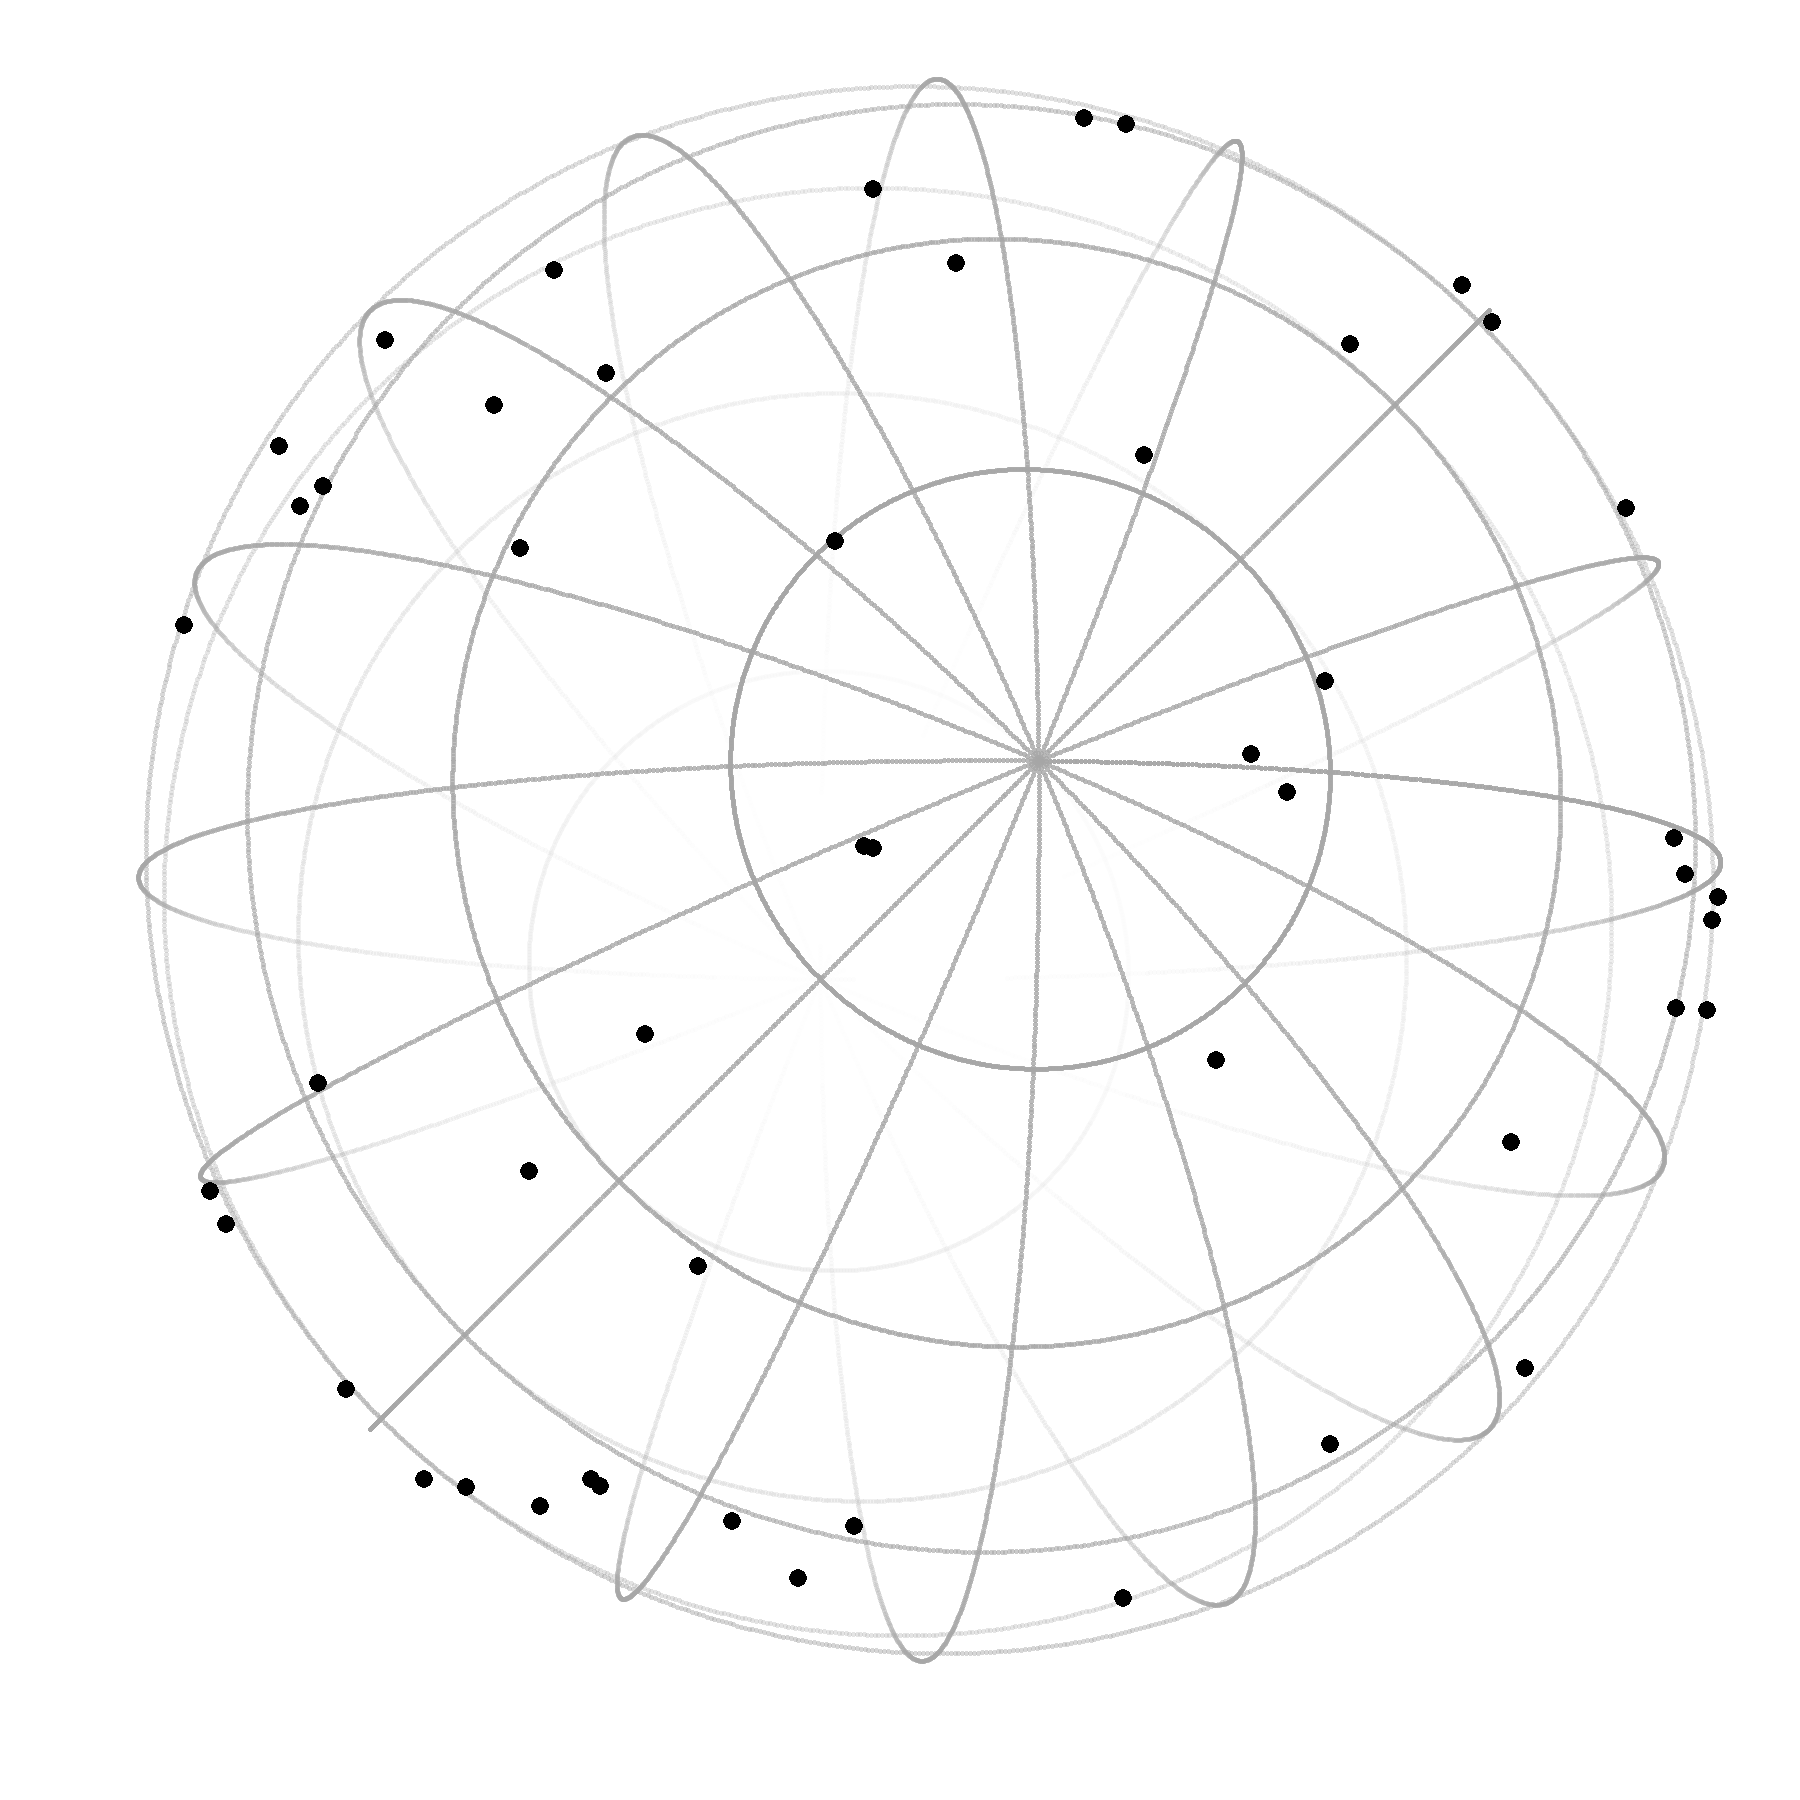
\includegraphics[width=\textwidth]{figures/eye1}
%		\caption{A random sample from the Cayley-UARS distribution with $\kappa=1$, $n=50$.}
%		\label{fig:sample}
%	\end{subfigure}
	\begin{subfigure}[h]{.45\textwidth}
		%\centering
		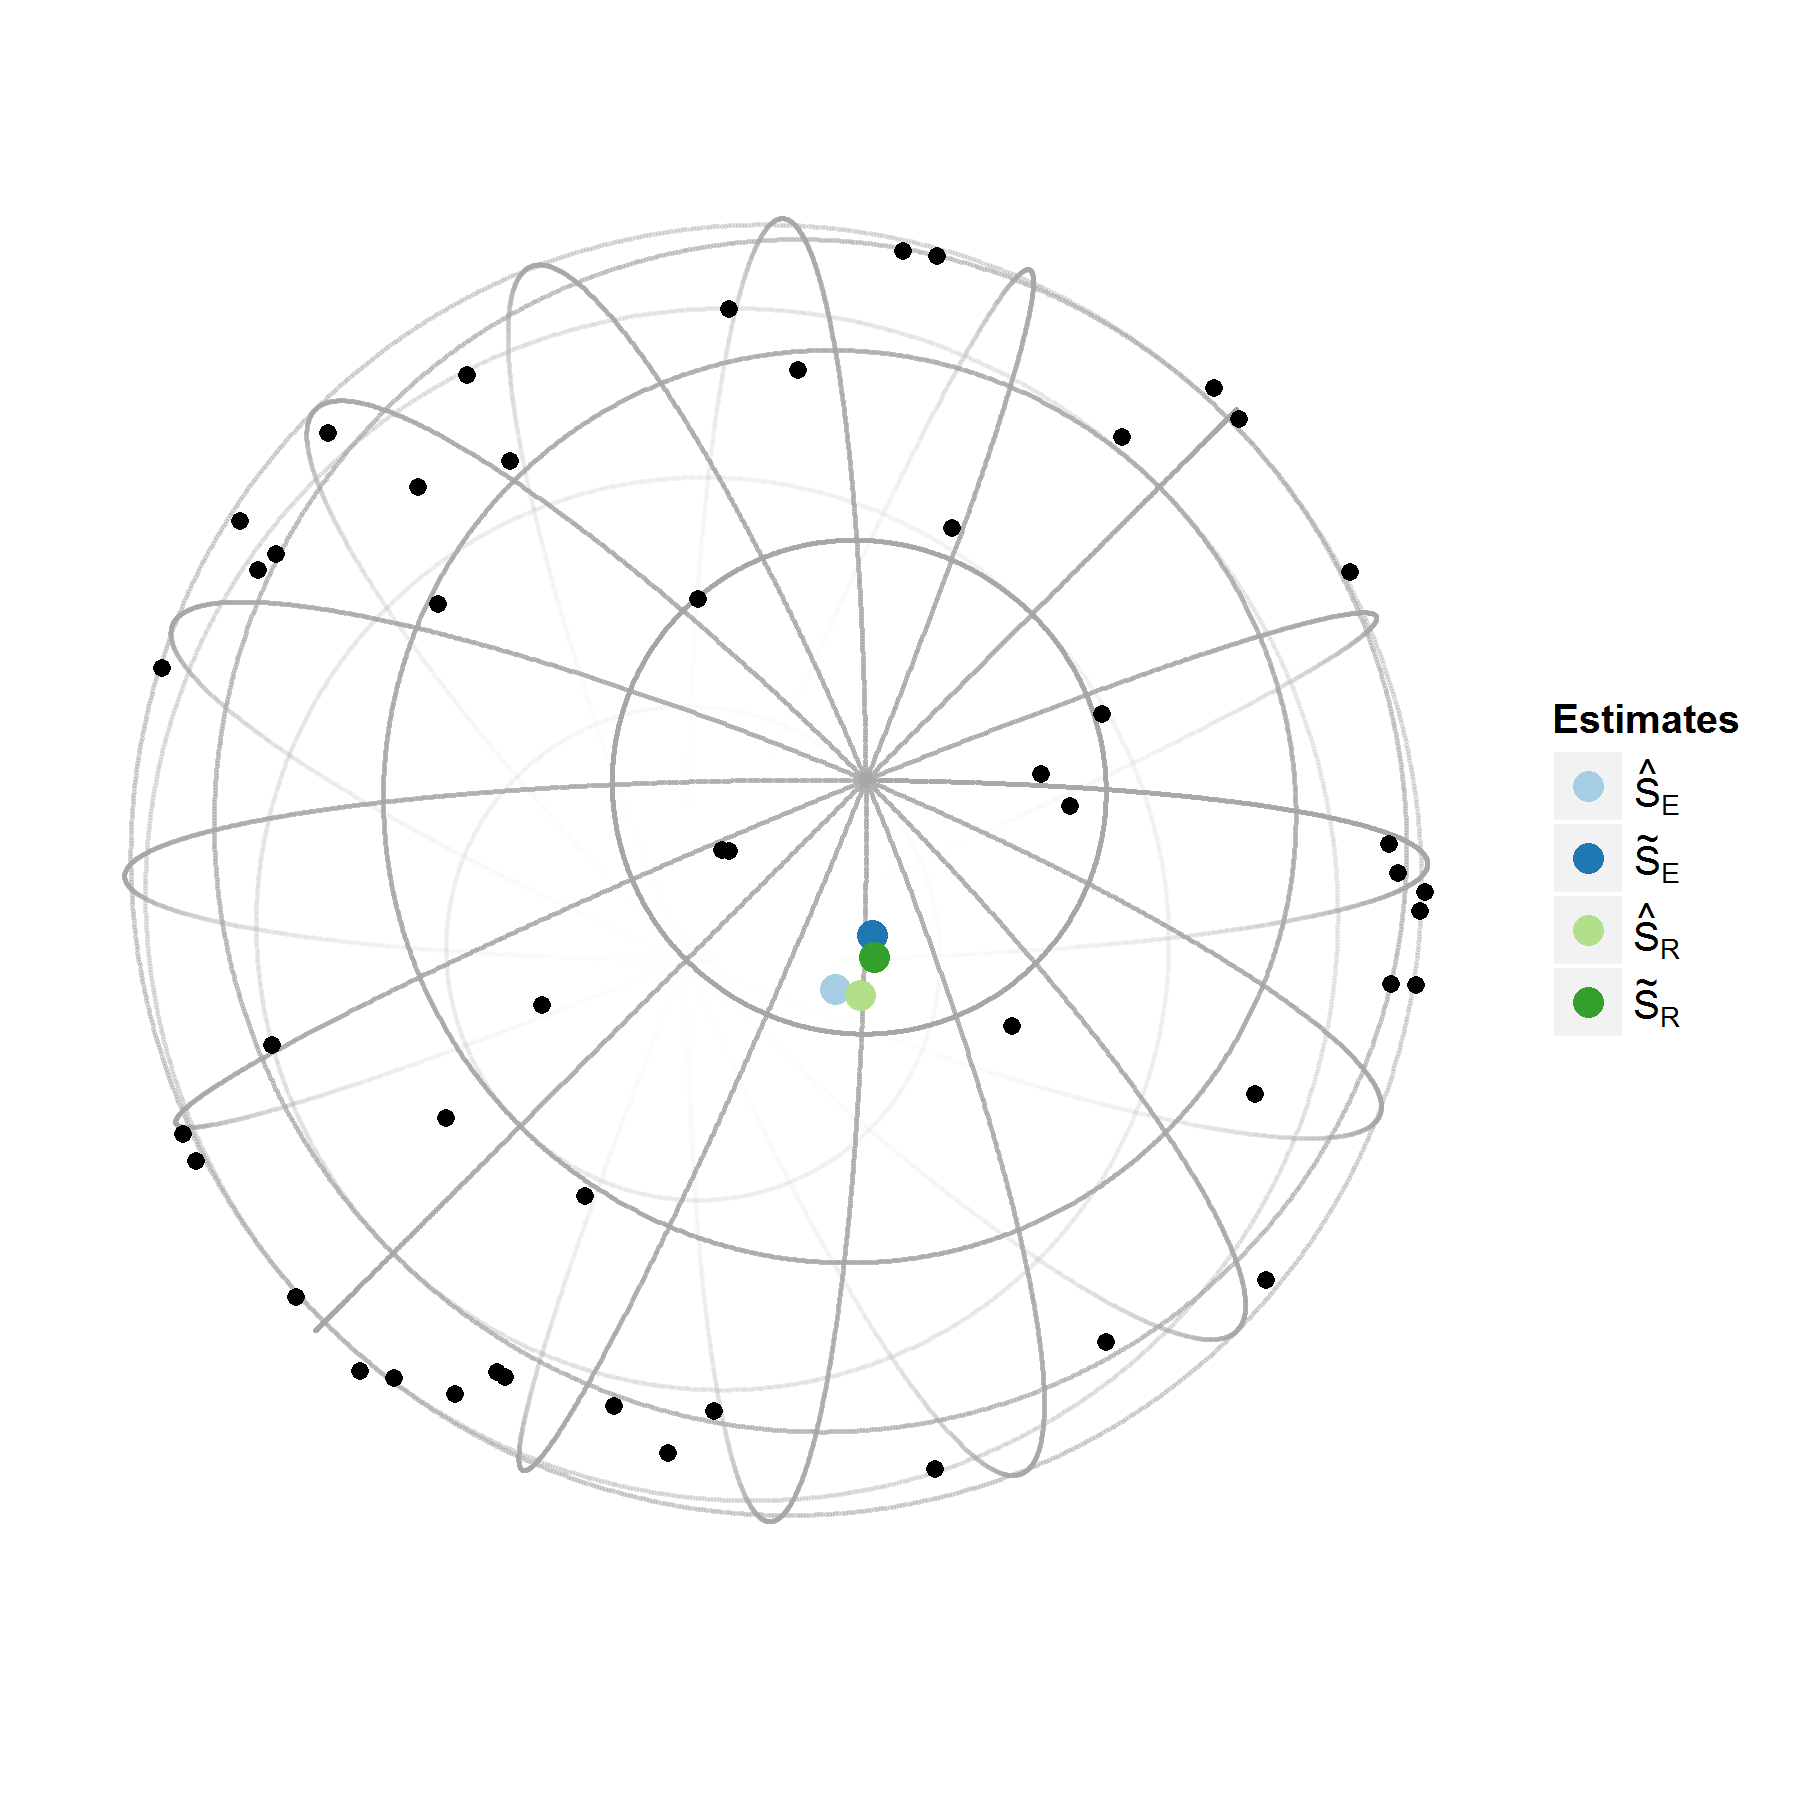
\includegraphics[width=\textwidth]{figures/eye2}
		\caption{Point estimates}
		\label{fig:ests}
	\end{subfigure}
	\begin{subfigure}[h]{.45\textwidth}
		%\centering
		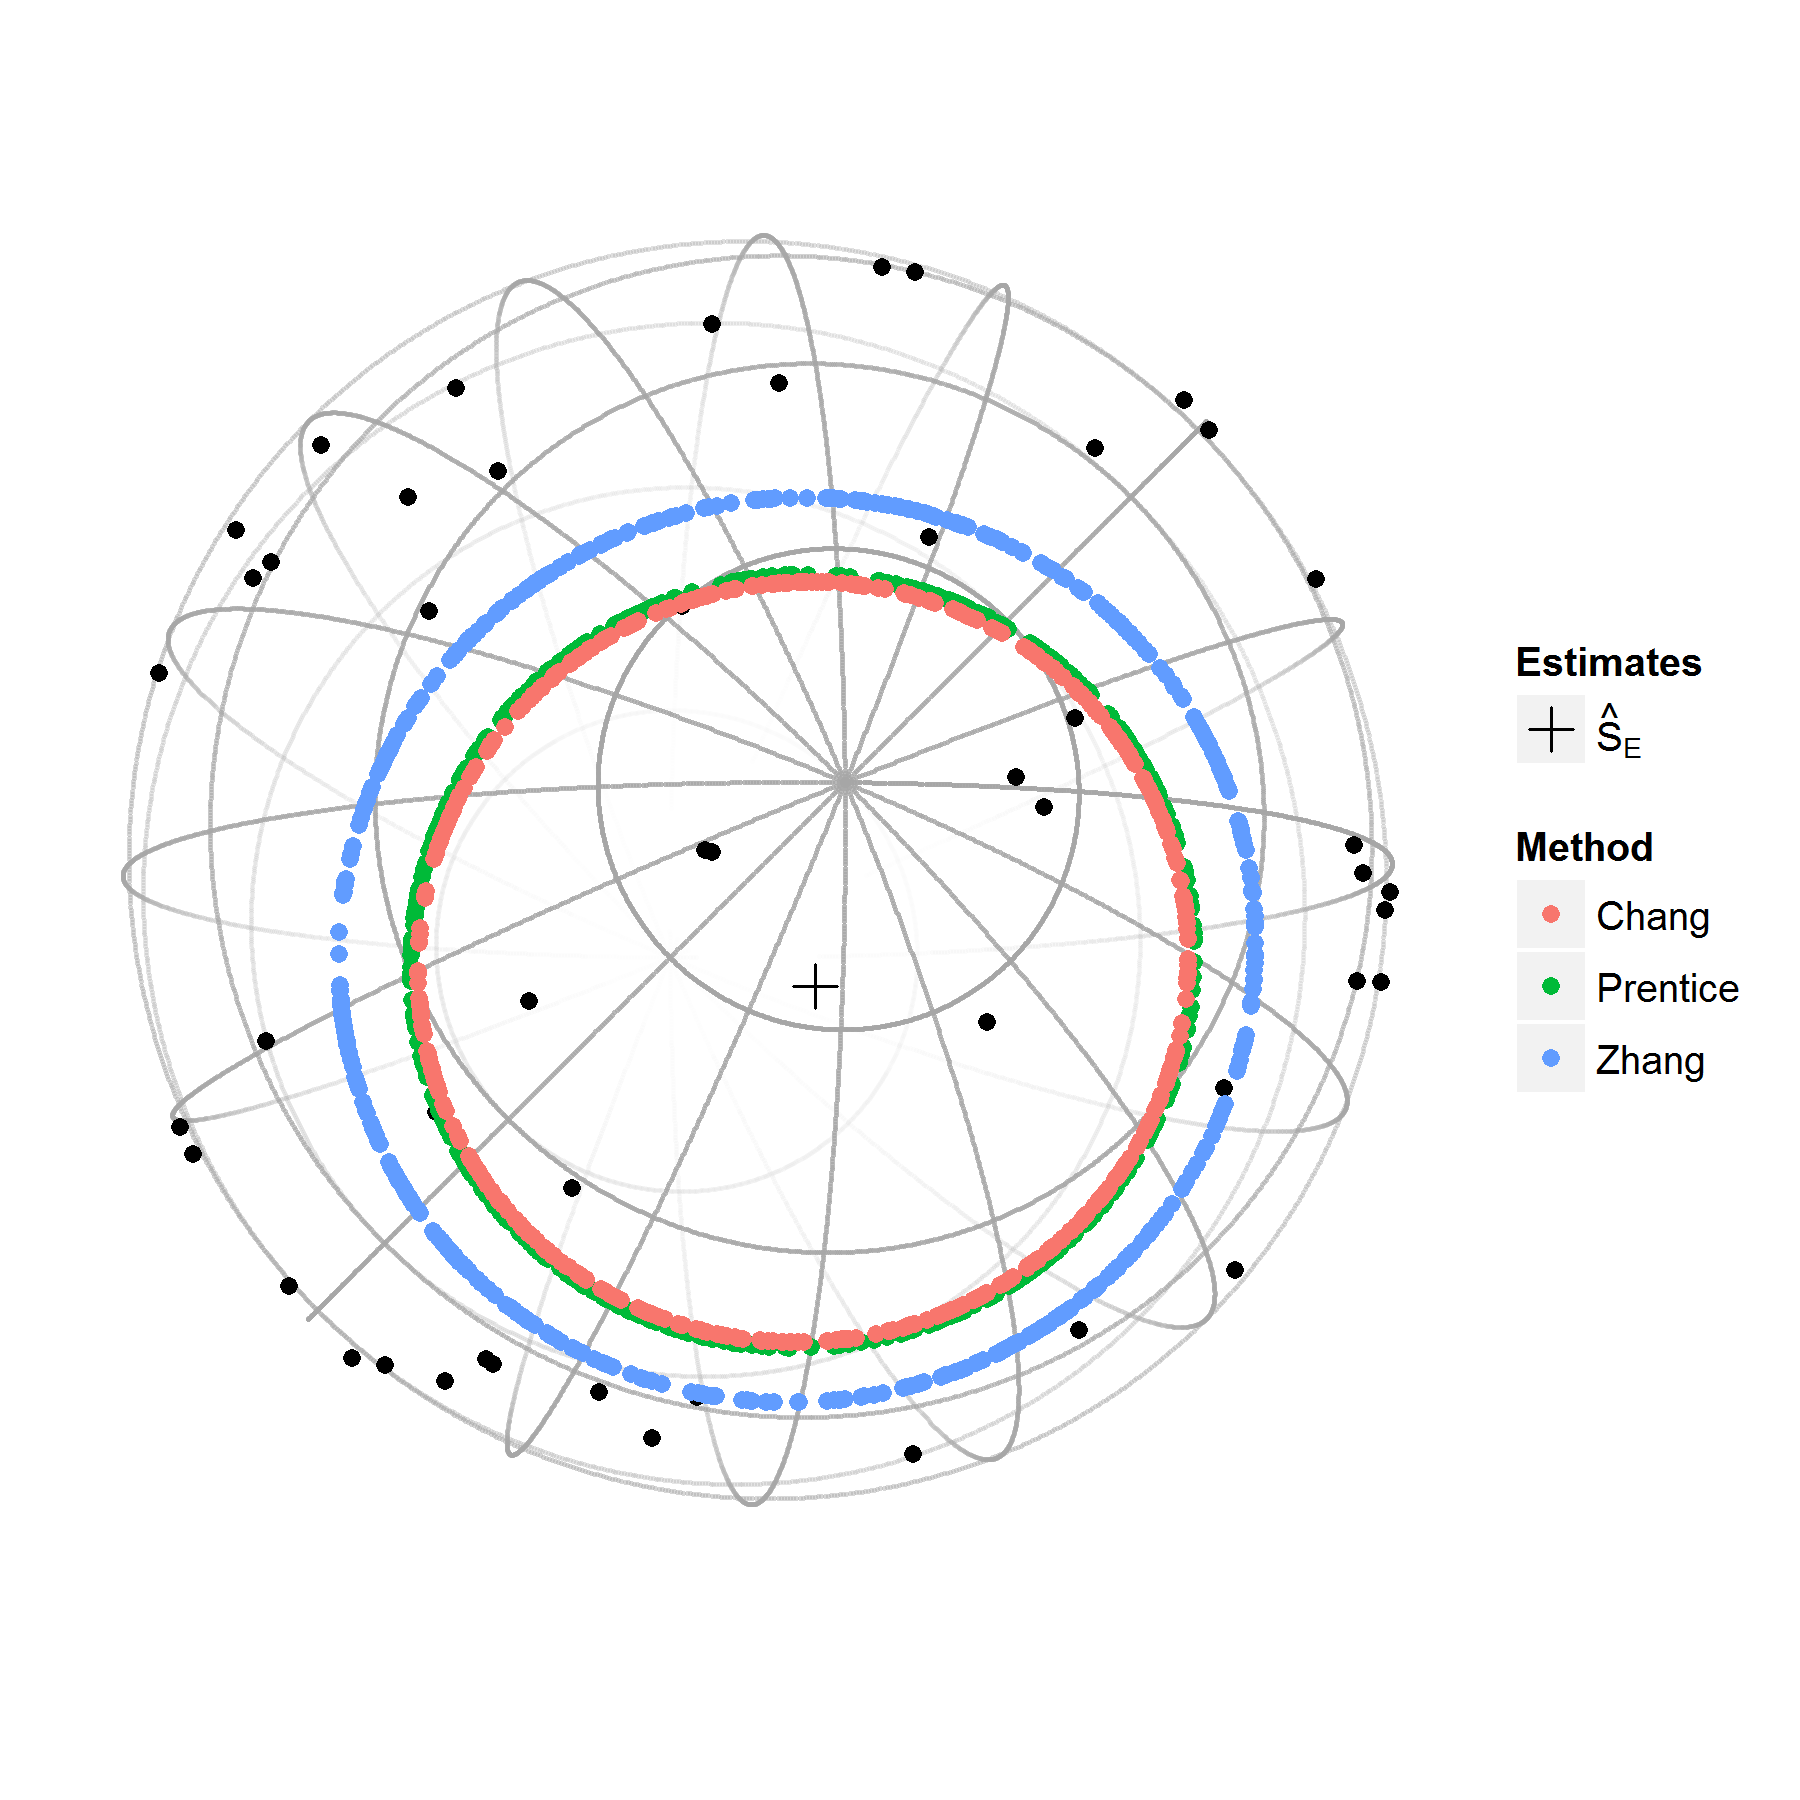
\includegraphics[width=\textwidth]{figures/eye3}
		\caption{Confidence region estimates}
		\label{fig:regs}
	\end{subfigure}
	
	\caption{\label{figure:eye1}The $x$-axis of a random sample from the Cayley-UARS distribution with $\kappa=1$, $n=50$.  All for point estimates are displayed in (a) and all three region methods along with the projected mean are in (b).}
	
\end{figure}

In Figure \ref{fig:ests} a random sample of 50 matrices following the Cayley-UARS distribution with $\kappa=1$ is plotted along with four estimates of the central orientation.  The confidence region methods and how they are displayed by the \code{plot} function is illustrated in Figure \ref{fig:regs}.

\section{Summary}

In this manuscript we introduced the \pkg{rotations} package and how it can be used to generate, analyze and visualize rotation data.  In future version of the package we plan to extend the parameterization and estimator sections including robust estimators that are currently being developed by the authors.  


\bibliography{stanfill-hofmann-genschel}

\address{Bryan Stanfill\\
  Department of Statistics\\
  Iowa State University\\
  Ames, IA 50011}\\
\email{stanfill@iastate.edu}

\address{Heike Hofmann\\
  Department of Statistics\\
  Iowa State University\\
  Ames, IA 50011}\\
\email{hofmann@mail.iastate.edu}

\address{Ulrike Genschel\\
  Department of Statistics\\
  Iowa State University\\
  Ames, IA 50011}\\
\email{ulrike@mail.iastate.edu}